% Source: Code/RADAR_web/docs/figures/fig_state_machine.tex
\documentclass[border=5pt]{standalone}
\usepackage{tikz}
\usetikzlibrary{arrows.meta,positioning}
\usepackage{xcolor}

\definecolor{garnet}{HTML}{73000A}
\definecolor{black10}{HTML}{ECECEC}
\definecolor{atlantic}{HTML}{466A9F}

\begin{document}
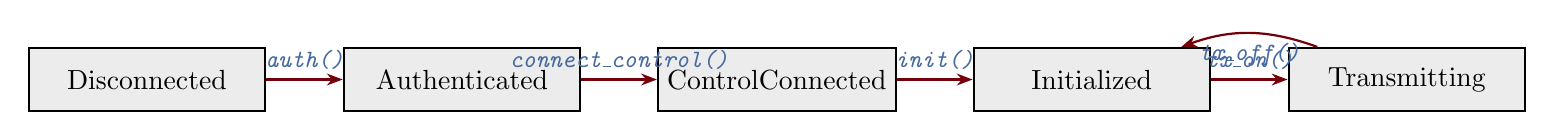
\begin{tikzpicture}[
    state/.style={draw, thick, minimum width=3cm, minimum height=0.8cm, align=center, fill=black10},
    trans/.style={-{Stealth[length=2mm]}, thick, color=garnet},
    label/.style={font=\small\itshape, color=atlantic, midway, above},
]

\node[state] (disc) at (0, 0) {Disconnected};
\node[state] (auth) at (4, 0) {Authenticated};
\node[state] (ctrl) at (8, 0) {ControlConnected};
\node[state] (init) at (12, 0) {Initialized};
\node[state] (tx) at (16, 0) {Transmitting};

\draw[trans] (disc) -- (auth) node[label] {\texttt{auth()}};
\draw[trans] (auth) -- (ctrl) node[label] {\texttt{connect\_control()}};
\draw[trans] (ctrl) -- (init) node[label] {\texttt{init()}};
\draw[trans] (init) -- (tx) node[label] {\texttt{tx\_on()}};
\draw[trans] (tx) to[bend right=20] node[font=\small\itshape, color=atlantic, midway, below] {\texttt{tx\_off()}} (init);

\end{tikzpicture}
\end{document}
